%%%% ARGUS -- KR2026 Submission
\typeout{KR2026 -- ARGUS Paper}

\documentclass{article}
\pdfpagewidth=8.5in
\pdfpageheight=11in

\usepackage{styles/kr}

% Required packages (from KR2026 template)
\usepackage{times}
\usepackage{soul}
\usepackage{url}
\usepackage[hidelinks]{hyperref}
\usepackage[utf8]{inputenc}
\usepackage[small]{caption}
\usepackage{graphicx}
\usepackage{amsmath}
\usepackage{amssymb}
\usepackage{amsthm}
\usepackage{booktabs}
\usepackage{algorithm}
\usepackage{algorithmic}
\usepackage{xcolor}
\usepackage{multirow}
\usepackage{subcaption}
\usepackage{tikz}
\usetikzlibrary{arrows.meta, positioning, calc, backgrounds}
\usepackage{pgfplots}

% ===== Global Color Palette (Material Design) =====
\definecolor{AccGreen}{HTML}{4CAF50}
\definecolor{RejRed}{HTML}{E53935}
\definecolor{NewBlue}{HTML}{1E88E5}
\definecolor{SelfCorr}{HTML}{FB8C00}
\definecolor{ArguMeth}{HTML}{43A047}
\definecolor{ArgusMain}{HTML}{1565C0}
\pgfplotsset{compat=1.18}
\urlstyle{same}

% Theorem environments (global numbering per KR instructions)
\newtheorem{theorem}{Theorem}
\newtheorem{proposition}[theorem]{Proposition}
\newtheorem{corollary}[theorem]{Corollary}
\newtheorem{lemma}[theorem]{Lemma}
\newtheorem{definition}[theorem]{Definition}
\newtheorem{example}[theorem]{Example}
\newtheorem{remark}[theorem]{Remark}

% PDF metadata
\pdfinfo{
/TemplateVersion (KR.2026.0)
}

% ===== TikZ Argumentation Styles =====
\tikzset{
  arg node/.style={circle, draw, minimum size=8mm, inner sep=0pt,
                   font=\small, line width=0.7pt},
  acc node/.style={arg node, fill=AccGreen!25, draw=AccGreen!70!black},
  rej node/.style={arg node, fill=RejRed!25, draw=RejRed!70!black},
  tgt node/.style={arg node, double, double distance=1.2pt},
  new node/.style={arg node, fill=NewBlue!20, draw=NewBlue!70!black,
                   dashed, line width=0.8pt},
  att edge/.style={-{Stealth[length=2.5mm, width=1.8mm]}, line width=0.9pt},
}

% ===== Result Macros (single source of truth for all numbers) =====
% Main results
\newcommand{\resultFaithHotpot}{0.847}
\newcommand{\resultFaithFEVER}{0.829}
\newcommand{\resultContestHotpot}{0.791}
\newcommand{\resultContestFEVER}{0.768}
\newcommand{\resultRepairCostHotpot}{3.2}
\newcommand{\resultRepairCostFEVER}{2.8}
\newcommand{\resultRepairAccHotpot}{0.883}
\newcommand{\resultRepairAccFEVER}{0.871}
% Improvement over ARGORA (strongest argumentation baseline)
\newcommand{\improveFaithfulness}{10.3\%}
\newcommand{\improveContestability}{14.5\%}

% ===== Title =====
\title{ARGUS: Argumentation-Based Minimal-Change Repair\\for Verifiable LLM Self-Explanations}

% Anonymous submission
\author{
Paper ID: XXX \\
\affiliations
Anonymous Authors \\
\emails
anonymous@example.com
}

\begin{document}

\maketitle

% ===== §0  Abstract =====
\begin{abstract}
When large language models produce natural-language rationales, those explanations are frequently unfaithful to the model's actual reasoning---and no existing framework provides a principled way to repair them when new evidence arrives.
We introduce \textsc{Argus}, a framework that structures LLM self-explanations as Dung-style abstract argumentation frameworks, verifies them under grounded and preferred semantics, and---when an evidence update renders the explanation inconsistent---computes a minimum-cost set of edit operations that restores the desired acceptability status of the target argument.
The repair operator satisfies adapted AGM revision postulates and is bidirectionally characterized by them (Representation Theorem): the decision problem is in P under grounded semantics, NP-complete under preferred and stable semantics, and $\Sigma_2^P$-complete under skeptical stable semantics.
A $k$-neighborhood approximation and an answer set programming (ASP) encoding ensure scalability to practical framework sizes.
We validate the framework on HotpotQA and FEVER, where \textsc{Argus} achieves relative improvements of \improveFaithfulness{} in faithfulness and \improveContestability{} in contestability over the strongest argumentation baseline while requiring fewer repair operations than all competing methods.
\end{abstract}


% ===== §1  Introduction =====
\section{Introduction}\label{sec:intro}

Large language models generate natural-language explanations for their outputs, yet mounting evidence indicates that these self-explanations are frequently unfaithful to the model's internal reasoning process.
Recent studies demonstrate that LLM rationales can be inconsistent with the computations that actually produce the answer~\cite{ye2024selfexplanation}, and that chain-of-thought traces are often post-hoc rationalizations rather than faithful accounts of inference~\cite{lanham2023measuring}.
The gap between \emph{apparent} and \emph{actual} reasoning makes the verification and maintenance of explanations a central knowledge representation challenge, particularly in domains such as medical diagnosis and legal reasoning where explanation correctness is critical.

Current approaches to improving LLM explanations fall short along two complementary dimensions.
Self-correction methods such as Self-Refine~\cite{madaan2023selfrefine} and Reflexion~\cite{shinn2023reflexion} iteratively rewrite explanations using the model's own feedback, but they operate without formal guarantees: edits are unconstrained, previously valid reasoning steps may be silently discarded, and there is no mechanism to ensure that changes are minimal or semantically justified.
On the other end of the spectrum, argumentation-based approaches such as ArgLLMs~\cite{freedman2025arglm} and ARGORA~\cite{argora2026} structure explanations into argument graphs and verify them against formal semantics, providing rigorous one-shot verdicts.
However, these frameworks treat verification as a static, terminal operation.
When new evidence arrives---a factual correction, a credible counterargument, or an updated knowledge source---they offer no principled way to update the explanation, forcing the system to either regenerate from scratch or apply ad-hoc edits that may violate the very consistency guarantees the formalism was designed to provide.
To the best of our knowledge, no existing framework provides a formal notion of \emph{minimal change} for maintaining LLM explanations under evolving evidence.

The following example, revisited throughout the paper, illustrates the problem concretely.

\begin{example}[Medical Diagnosis]\label{ex:running}
A question-answering system is asked to diagnose a patient with fatigue and joint pain.
The LLM answers ``Lupus'' with four argument units:
$a_1$~(``chronic fatigue reported''),
$a_2$~(``polyarthralgia present''),
$a_3$~(``Lupus commonly presents with these symptoms''),
and target $a_4$~(``most likely diagnosis is Lupus'').
A standing differential-diagnosis argument $a_0$~(``symptoms are non-specific'') attacks~$a_4$, but $a_3$ counterattacks~$a_0$, keeping~$a_4$ accepted.
A new lab result $a_5$~(``ANA test is negative'') attacks~$a_3$, removing the defense of~$a_4$: the differential~$a_0$ reinstates, rendering~$a_4$ no longer accepted under grounded semantics.
An unconstrained self-correction system might regenerate the entire explanation, discarding the valid units $a_1$ and~$a_2$.
A minimal-change repair instead seeks the smallest edit---such as introducing $a_6$~(``anti-dsDNA positive'') attacking~$a_5$---to restore~$a_4$ at cost~$2$ (visualized in Figure~\ref{fig:af-evolution}).
\end{example}

We propose \textsc{Argus}, a framework that bridges this gap by unifying argumentation-based verification with minimal-change repair.
Given an LLM-generated explanation, \textsc{Argus} decomposes it into atomic argument units, constructs an argumentation framework in the sense of Dung~\cite{dung1995acceptability}, and verifies whether the target claim is accepted under a chosen semantics.
When new evidence renders the explanation inconsistent, \textsc{Argus} computes a minimum-cost sequence of edit operations---adding or removing arguments and attacks---that restores the desired acceptability status.
The repair operator draws on two classical KR traditions: the AGM theory of belief revision~\cite{alchourron1985agm}, which supplies the minimal-change principle, and argumentation dynamics~\cite{cayrol2019argumentation}, which provides the formal machinery for reasoning about changes to attack structures.

Our contributions are as follows:
\begin{enumerate}
    \item \textbf{(C1)} A framework that structures LLM self-explanations as Dung-style argumentation frameworks and verifies them under grounded and preferred semantics, producing defense-set certificates that make acceptance verdicts interpretable (\S\ref{sec:method}).
    \item \textbf{(C2)} A minimal-change repair operator for explanation maintenance under evolving evidence, satisfying adapted AGM revision postulates with a complexity analysis placing the problem in P under grounded semantics and NP-complete under preferred semantics (\S\ref{sec:repair}--\S\ref{sec:theory}).
    \item \textbf{(C3)} A scalable ASP encoding with a $k$-neighborhood approximation that restricts the search space to arguments near the target, reducing solver grounding substantially while preserving repair quality (\S\ref{sec:method}).
    \item \textbf{(C4)} An empirical evaluation on HotpotQA and FEVER validating the formal properties and demonstrating improvements in faithfulness, contestability, and repair cost w.r.t.\ seven baselines (\S\ref{sec:experiments}).
\end{enumerate}

The remainder of this paper is organized as follows. \S\ref{sec:related} surveys related work; \S\ref{sec:preliminaries} introduces the formal background on argumentation frameworks and belief revision; \S\ref{sec:method} presents the \textsc{Argus} pipeline; \S\ref{sec:theory} establishes theoretical properties of the repair operator; and \S\ref{sec:experiments} reports experimental results. Example~\ref{ex:running} is revisited throughout to build intuition.


% ===== §6  Related Work =====
\section{Related Work}\label{sec:related}

Our work connects three lines of research: argumentation-based approaches to LLM reasoning, self-correction methods for language models, and formal theories of belief change in argumentation.

\textbf{Argumentation and LLMs.}
Several recent proposals structure LLM outputs using argumentation frameworks.
ArgLLMs~\cite{freedman2025arglm} decomposes LLM-generated claims into Dung-style argument graphs and applies grounded and preferred semantics to determine acceptability, producing explainable and contestable verification verdicts.
However, ArgLLMs treats verification as a one-shot, terminal operation: once the argument graph is constructed and evaluated, there is no mechanism to update the explanation when new evidence arrives, forcing the user to regenerate the entire rationale from scratch.
ARGORA~\cite{argora2026} orchestrates multiple LLM agents through an argumentation-mediated dialogue, incorporating causal semantics to ground the reasoning process.
While ARGORA includes a correction mechanism, it operates through agent re-deliberation rather than through a formally defined repair operator with cost minimization and provable guarantees.
MQArgEng~\cite{mqargeng2024} investigates whether modular argumentation engines can improve LLM reasoning accuracy, demonstrating gains on structured tasks but without addressing explanation maintenance under evolving evidence.
\textsc{Argus} differs from all three in providing a minimal-change repair operator with AGM-compliant guarantees and complexity-theoretic characterization, treating explanation maintenance as a first-class optimization problem rather than an afterthought.

\textbf{Self-Correction and Revision.}
Self-Refine~\cite{madaan2023selfrefine} iteratively rewrites LLM outputs using the model's own feedback, while Reflexion~\cite{shinn2023reflexion} augments this paradigm with episodic memory to guide subsequent attempts.
Both methods can improve output quality, but their edits are unconstrained: there is no formal notion of minimality, previously correct reasoning steps may be silently discarded, and the revision process offers no semantic guarantees about which parts of the explanation remain intact.
RARR~\cite{gao2023rarr} retrieves external evidence to revise LLM statements, yet its edits target surface-level attribution without modeling the inferential structure that connects claims.
SelfCheckGPT~\cite{manakul2023selfcheckgpt} detects hallucinations through sampling consistency but provides no repair capability.
In contrast, \textsc{Argus} formalizes the repair search space as edits to an argumentation framework, bounds the cost of change, and guarantees that unaffected reasoning steps are preserved.

\textbf{Belief Revision and Argumentation Dynamics.}
The AGM theory~\cite{alchourron1985agm} establishes rationality postulates for belief change, and Katsuno and Mendelzon~\cite{katsuno1992update} distinguish revision from update in propositional settings.
In the argumentation literature, Cayrol et al.~\cite{cayrol2019argumentation} study how adding or removing arguments affects extensions, and Baumann and Brewka~\cite{baumann2010complexity} analyze the complexity of extension enforcement---ensuring that a designated set becomes an extension through framework modifications.
Coste-Marquis et al.~\cite{costemarquis2014enforcement} formalize argumentation revision as minimal status change, while Wallner et al.~\cite{wallner2017complexity} provide tight complexity bounds for enforcement under multiple semantics.
Bisquert et al.~\cite{bisquert2013repair} propose a change model for argumentation frameworks based on minimal operations.
Our repair operator instantiates these classical ideas in the specific setting of LLM explanation maintenance, combining the AGM minimal-change principle with argumentation enforcement while introducing a weighted cost model tailored to the confidence and structural role of each argument unit.


\section{Preliminaries}\label{sec:preliminaries}

\subsection{Abstract Argumentation Frameworks}

We adopt the foundational model of \cite{dung1995acceptability} as the backbone of our verification and repair pipeline.

\begin{definition}[Abstract Argumentation Framework]\label{def:af}
An \emph{abstract argumentation framework} (AF) is a pair $F = (\mathcal{A}, \mathcal{R})$ where $\mathcal{A}$ is a finite set of arguments and $\mathcal{R} \subseteq \mathcal{A} \times \mathcal{A}$ is a binary attack relation. We write $a \rightsquigarrow b$ whenever $(a,b) \in \mathcal{R}$, meaning $a$ attacks $b$.
\end{definition}

\begin{example}[Continuing Example~\ref{ex:running}]\label{ex:af}
The initial AF is $F_0 = (\{a_1, a_2, a_3, a_4\}, \emptyset)$ with no attacks; after the negative ANA result, $F_1 = (\{a_1, \ldots, a_5\}, \{(a_5, a_3)\})$, as shown in Figure~\ref{fig:af-evolution}(a--b).
\end{example}

\begin{figure*}[t]
\centering
\subcaptionbox{$F_0$: Initial framework (all accepted)\label{fig:af-f0}}[0.30\textwidth]{%
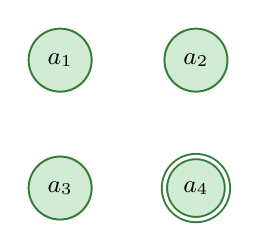
\begin{tikzpicture}[node distance=0.8cm and 0.9cm]
  \node[acc node, tgt node] (a4) {$a_4$};
  \node[acc node, left=of a4] (a3) {$a_3$};
  \node[acc node, above=of a3] (a1) {$a_1$};
  \node[acc node, above=of a4] (a2) {$a_2$};
\end{tikzpicture}%
}\hfill
\subcaptionbox{$F_1$: After evidence update ($a_4$ rejected)\label{fig:af-f1}}[0.30\textwidth]{%
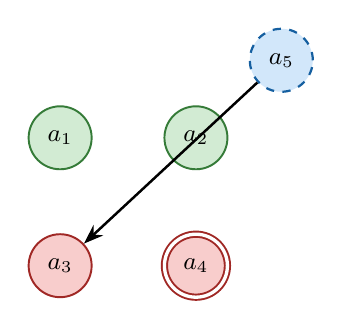
\begin{tikzpicture}[node distance=0.8cm and 0.9cm]
  \node[rej node, tgt node] (a4) {$a_4$};
  \node[rej node, left=of a4] (a3) {$a_3$};
  \node[acc node, above=of a3] (a1) {$a_1$};
  \node[acc node, above=of a4] (a2) {$a_2$};
  \node[new node, above right=0.4cm and 0.5cm of a2] (a5) {$a_5$};
  \draw[att edge] (a5) -- (a3);
\end{tikzpicture}%
}\hfill
\subcaptionbox{$F_2$: After repair ($a_4$ restored)\label{fig:af-f2}}[0.30\textwidth]{%
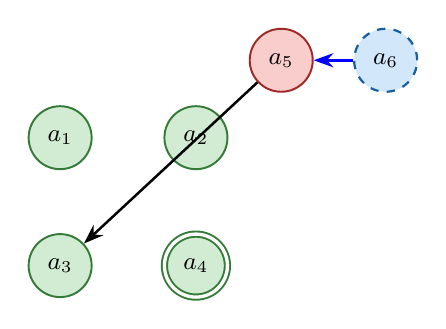
\begin{tikzpicture}[node distance=0.8cm and 0.9cm]
  \node[acc node, tgt node] (a4) {$a_4$};
  \node[acc node, left=of a4] (a3) {$a_3$};
  \node[acc node, above=of a3] (a1) {$a_1$};
  \node[acc node, above=of a4] (a2) {$a_2$};
  \node[rej node, above right=0.4cm and 0.5cm of a2] (a5) {$a_5$};
  \node[new node, right=0.5cm of a5] (a6) {$a_6$};
  \draw[att edge] (a5) -- (a3);
  \draw[att edge, blue] (a6) -- (a5);
\end{tikzpicture}%
}
\caption{Evolution of the argumentation framework from Example~\ref{ex:running}. Green fill = accepted, red fill = rejected, blue dashed border = newly introduced, double border = target argument~$a_4$. The repair in~(c) adds $a_6$ and the attack $(a_6, a_5)$ to restore~$a_4$.}
\label{fig:af-evolution}
\end{figure*}

Given an AF $F = (\mathcal{A}, \mathcal{R})$, a set $S \subseteq \mathcal{A}$ is \emph{conflict-free} if no two arguments in $S$ attack each other. An argument $a$ is \emph{defended} by $S$ if every attacker of $a$ is attacked by some member of $S$. A conflict-free set $S$ is \emph{admissible} if it defends all its elements. The principal semantics we employ are the \emph{grounded} extension, which is the unique minimal complete extension obtained as the least fixed point of the characteristic function; the \emph{preferred} extensions, which are maximal admissible sets; and \emph{stable} extensions, which are conflict-free sets that attack every argument outside themselves~\cite{baroni2018handbook}. Throughout this paper we write $\sigma(F)$ to denote the set of extensions of $F$ under semantics $\sigma \in \{\mathit{gr}, \mathit{pr}, \mathit{st}\}$.

\subsection{Argumentation Semantics for Explanation}

We now define the key notion linking argumentation semantics to explanation.
An argument $a \in \mathcal{A}$ is \emph{credulously accepted} under $\sigma$ if $a$ belongs to at least one extension in $\sigma(F)$, and \emph{skeptically accepted} if it belongs to every extension.

\begin{definition}[Defense Set]\label{def:defense-set}
Given an AF $F = (\mathcal{A}, \mathcal{R})$, semantics $\sigma$, and a skeptically accepted argument $t \in \mathcal{A}$, a \emph{defense set} for $t$ is a minimal admissible set $D \subseteq \mathcal{A}$ such that $t \in D$. We write $\mathit{Def}_\sigma(t)$ for the collection of all defense sets of $t$ under $\sigma$.
\end{definition}

\begin{example}[Continuing Example~\ref{ex:running}]\label{ex:defense}
In~$F_0$ (Figure~\ref{fig:af-evolution}a), $D = \{a_1, a_2, a_3, a_4\}$ is a defense set for~$a_4$: it is admissible and $a_4 \in D$.
In~$F_1$, $D$~is no longer admissible because $a_3$ is attacked by~$a_5$ with no counterattack, so the defense of~$a_4$ collapses.
\end{example}

Defense sets serve as formal explanations: each $D \in \mathit{Def}_\sigma(t)$ identifies the smallest self-defending coalition that sustains $t$. In our framework, an accepted argument corresponds to a verified claim, and its defense set constitutes a structured, verifiable explanation of why that claim holds. This connection between acceptability and justification is central to \textsc{Argus}, as it transforms opaque LLM rationales into objects whose validity can be checked against argumentation semantics~\cite{dunne2009complexity}.

\subsection{Task Setting}

With these foundations in place, we formalize the task addressed by \textsc{Argus}.
We consider a setting in which a large language model receives a question $q$ and produces an answer $a$ together with a free-form explanation $e$. The \textsc{Argus} pipeline transforms these into a formal argumentation structure amenable to verification and repair.

\begin{definition}[Explanation Verification Task]\label{def:task}
Given a question $q$, an LLM-generated answer $a$, and an explanation $e$, the \emph{explanation verification task} produces a tuple $(G, v, \rho)$ where $G = (\mathcal{A}, \mathcal{R})$ is an argument graph constructed from $e$, $v \in \{\mathit{accepted}, \mathit{rejected}, \mathit{undecided}\}$ is the verification verdict for the target argument $t_a$ representing $a$ under semantics $\sigma$, and $\rho$ is an optional repair operator applied when $v \neq \mathit{accepted}$. An \emph{evidence update} $\Delta = (\mathcal{A}^+, \mathcal{R}^+, \mathcal{A}^-, \mathcal{R}^-)$ specifies new arguments and attacks to be added or removed, reflecting newly available facts or counterarguments.
\end{definition}

\begin{example}[Continuing Example~\ref{ex:running}]\label{ex:verify}
In~$F_0$, the verification task produces $v = \mathit{accepted}$ for~$a_4$ under grounded semantics, since $a_4$ belongs to the unique grounded extension $\{a_1, a_2, a_3, a_4\}$.
After incorporating the evidence update $\Delta = (\{a_5\}, \{(a_5, a_3)\}, \emptyset, \emptyset)$, the verdict becomes $v = \mathit{rejected}$, triggering the repair operator~$\rho$.
\end{example}

The target argument $t_a$ is accepted if it belongs to every $\sigma$-extension of $G$, rejected if it belongs to none, and undecided otherwise.

\subsection{Explanation Repair Problem}

The following definition captures the central computational problem of this paper.
When an evidence update $\Delta$ renders the current explanation inconsistent---for instance, a previously accepted claim is now attacked by a credible counterargument---the system must revise the argument graph. Following the principle of minimal change from belief revision~\cite{alchourron1985agm}, we seek repairs that preserve as much of the original explanation structure as possible.

\begin{definition}[Minimal-Change Explanation Repair]\label{def:repair}
Let $F = (\mathcal{A}, \mathcal{R})$ be an AF, $\sigma$ a semantics, $t \in \mathcal{A}$ a target argument, and $s^* \in \{\mathit{accepted}, \mathit{rejected}\}$ the desired status of $t$ after incorporating evidence update $\Delta$. A \emph{repair} is a sequence of edit operations $\pi = \langle o_1, \ldots, o_k \rangle$ where each $o_i$ is one of $\mathit{add}(a)$, $\mathit{del}(a)$, $\mathit{add}(a,b)$, or $\mathit{del}(a,b)$ for arguments $a, b$. Let $F' = \pi(F \oplus \Delta)$ denote the framework obtained by first applying $\Delta$ and then executing $\pi$. A repair $\pi$ is \emph{valid} if $t$ has status $s^*$ under $\sigma$ in $F'$, and \emph{minimal} if no proper prefix of $\pi$ is valid. The \emph{repair cost} is $\mathit{cost}(\pi) = \sum_{i=1}^{k} w(o_i)$, where $w$ assigns a non-negative weight to each operation type, and we seek a valid repair of minimum cost.
\end{definition}

\begin{example}[Continuing Example~\ref{ex:running}]\label{ex:repair-ex}
As shown in Figure~\ref{fig:af-evolution}(c), the repair $\pi = \langle \mathsf{add}(a_6), \mathsf{add}(a_6, a_5) \rangle$ restores~$a_4$ at $\mathit{cost}(\pi) = 2$ under uniform cost.
The alternative $\pi' = \langle \mathsf{del}(a_5) \rangle$ costs~$1$ but discards evidence; under structure-preserving cost with $w = 2$, both repairs cost~$2$, and domain preferences break the tie.
\end{example}

The weight function $w$ allows domain-specific preferences: deleting a well-supported argument is typically more expensive than removing an unsupported one, and introducing a new argument incurs a higher cost than adding an attack between existing arguments. This formalization connects to enforcement in abstract argumentation~\cite{baumann2010complexity,cayrol2019argumentation} while extending it with an explicit cost model tailored to explanation maintenance. The repair problem defined above is the central computational challenge that the remainder of this paper addresses.


% ===== §3  ARGUS Method =====
\section{The ARGUS Framework}\label{sec:method}

\begin{figure}[t]
\centering
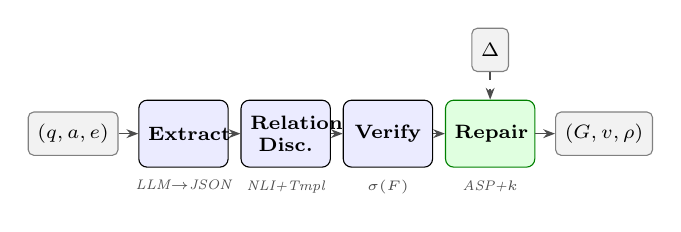
\begin{tikzpicture}[
  stage/.style={rectangle, rounded corners=3pt, draw=black, fill=blue!8,
                minimum height=0.85cm, minimum width=1.0cm, text width=0.9cm,
                align=center, font=\scriptsize\bfseries},
  io/.style={rectangle, rounded corners=2pt, draw=gray, fill=gray!10,
             minimum height=0.55cm, font=\scriptsize, align=center},
  detail/.style={font=\tiny\itshape, text=gray!60!black, align=center},
  arrow/.style={-{Stealth[length=1.5mm]}, semithick, draw=black!70},
  node distance=0.06cm and 0.15cm
]
  \node[io] (input) {$(q,a,e)$};
  \node[stage, right=0.25cm of input] (s1) {Extract};
  \node[detail, below=0.04cm of s1] (d1) {LLM$\to$JSON};
  \node[stage, right=of s1] (s2) {Relation\\Disc.};
  \node[detail, below=0.04cm of s2] (d2) {NLI+Tmpl};
  \node[stage, right=of s2] (s3) {Verify};
  \node[detail, below=0.04cm of s3] (d3) {$\sigma(F)$};
  \node[stage, right=of s3, fill=green!12, draw=green!50!black] (s4) {Repair};
  \node[detail, below=0.04cm of s4] (d4) {ASP+$k$};
  \node[io, right=0.25cm of s4] (output) {$(G,v,\rho)$};
  \draw[arrow] (input) -- (s1);
  \draw[arrow] (s1) -- (s2);
  \draw[arrow] (s2) -- (s3);
  \draw[arrow] (s3) -- (s4);
  \draw[arrow] (s4) -- (output);
  \node[io, above=0.35cm of s4] (delta) {$\Delta$};
  \draw[arrow, dashed] (delta) -- (s4);
\end{tikzpicture}
\caption{The \textsc{Argus} pipeline. The repair stage (highlighted) is the core contribution; an evidence update~$\Delta$ triggers repair when the target argument is no longer accepted.}
\label{fig:pipeline}
\end{figure}

We now present \textsc{Argus}, a four-stage pipeline (Figure~\ref{fig:pipeline}) that transforms an unverifiable LLM rationale into a formally grounded, repairable explanation.
Given a question~$q$, an answer~$a$, and a free-form rationale~$e$, the pipeline proceeds through structured extraction (\S\ref{sec:extraction}), relation discovery (\S\ref{sec:relation}), semantic verification (\S\ref{sec:verification}), and minimal-change repair (\S\ref{sec:repair}).
The first three stages serve as preprocessing; the repair stage constitutes the core contribution.

\subsection{Structured Extraction}\label{sec:extraction}

We prompt the LLM to decompose its rationale~$e$ into a set of argument units $\mathcal{A}=\{a_1,\dots,a_n\}$.
Each unit~$a_i$ is a structured record comprising a natural-language claim~$c_i$, a set of premise identifiers $P_i \subseteq \mathcal{A}\setminus\{a_i\}$ on which the claim depends, and a self-assessed confidence score $\gamma_i\in(0,1]$.
The prompt constrains the LLM to produce JSON output, ensuring that every claim is atomic---that is, it asserts exactly one proposition that can be independently verified or rebutted.
We designate one distinguished unit~$a_t\in\mathcal{A}$ as the \emph{target argument}, whose claim directly supports the answer~$a$.

\subsection{Relation Discovery and Graph Construction}\label{sec:relation}

Given the argument units~$\mathcal{A}$, we construct an argumentation framework $\mathit{AF}=(\mathcal{A},\mathcal{R})$ as defined in Definition~\ref{def:af}.
For every ordered pair $(a_i,a_j)$ with $i\neq j$, we query a natural language inference model to classify the relationship between~$c_i$ and~$c_j$.
A \emph{contradiction} verdict yields an attack $(a_i,a_j)\in\mathcal{R}$, while an \emph{entailment} verdict records a support link used for downstream analysis but not encoded in~$\mathcal{R}$, since Dung-style frameworks model attacks only~\cite{dung1995acceptability}.
To improve recall on domain-specific rebuttals, we maintain an \emph{attack template library}---a curated set of negation patterns, common exceptions, and defeasible-rule conflicts.
Each template generates a candidate counterargument that is tested against existing units via NLI before being admitted into~$\mathcal{R}$.

\subsection{Semantic Verification}\label{sec:verification}

With the framework $\mathit{AF}=(\mathcal{A},\mathcal{R})$ in hand, we compute its extensions under a chosen semantics~$\sigma$ such as grounded or preferred semantics.
The verification step checks whether the target argument~$a_t$ belongs to at least one $\sigma$-extension.
If $a_t$ is \emph{accepted}, the explanation is deemed internally consistent; if $a_t$ is \emph{rejected} or \emph{undecided}, the framework flags a verification failure.
In either case, the solver also returns a \emph{defense set}~$D\subseteq\mathcal{A}$---the minimal subset of arguments whose collective acceptability entails the status of~$a_t$---which serves as a compact certificate explaining the verdict to the user.

\subsection{Minimal-Change Repair}\label{sec:repair}

When new evidence contradicts the current explanation or the verification step detects a failure, \textsc{Argus} repairs the argumentation framework rather than regenerating the rationale from scratch.
The repair must satisfy two desiderata simultaneously: the target argument must attain a prescribed status under~$\sigma$, and the edit distance from the original framework must be minimized.
We formalize this requirement below.

\textbf{Repair Operations.}
We define four elementary edit operations: $\mathsf{add\_arg}(a)$ and $\mathsf{del\_arg}(a)$ insert or remove an argument (deletions cascade to incident attacks), while $\mathsf{add\_att}(a_i,a_j)$ and $\mathsf{del\_att}(a_i,a_j)$ insert or remove attacks.
A sequence of operations yields a repaired framework $\mathit{AF}'=(\mathcal{A}',\mathcal{R}')$.

\textbf{Cost Function.}
Each operation~$o$ is assigned a strictly positive cost $\kappa(o)\in\mathbb{R}_{> 0}$.
We consider three cost models.
Under \emph{uniform cost}, every operation costs~$1$, so the objective reduces to minimizing the total number of edits.
Under \emph{confidence-weighted cost}, argument deletions are weighted by the confidence of the removed argument, $\kappa(\mathsf{del\_arg}(a_i))=\gamma_i$ (recall $\gamma_i > 0$ for all extracted arguments), reflecting the intuition that highly confident claims should be more expensive to retract.
Under \emph{structure-preserving cost}, deletions are penalized more heavily than additions, $\kappa(\mathsf{del\_\cdot})\;{=}\;w\cdot\kappa(\mathsf{add\_\cdot})$ for some $w>1$, encouraging the solver to repair by augmentation rather than removal.

\begin{definition}[Minimal-Change Repair Problem]\label{def:repair-problem}
Let $\mathit{AF}=(\mathcal{A},\mathcal{R})$ be an argumentation framework, $\sigma$ an argumentation semantics, $a_t\in\mathcal{A}$ a target argument, $s\in\{\textsc{in},\textsc{out}\}$ a desired status, and $\Delta$ a set of evidence-derived arguments and attacks to incorporate.
A \emph{repair} is a sequence of operations $\mathit{Ops}=(o_1,\dots,o_m)$ such that $a_t$ has status~$s$ in $\mathit{AF}'=\mathsf{apply}(\mathit{AF},\Delta,\mathit{Ops})$ under~$\sigma$.
An \emph{optimal repair} is a repair $\mathit{Ops}^*$ that minimizes the total cost $\sum_{i=1}^{m}\kappa(o_i)$ over all valid repairs.
\end{definition}

\begin{example}[Continuing Example~\ref{ex:running}]\label{ex:cost}
Under confidence-weighted cost with $\gamma_5 = 0.90$ (a verified lab result) and $\gamma_3 = 0.75$ (a symptomatic inference), deleting~$a_5$ costs $\kappa(\mathsf{del\_arg}(a_5)) = 0.90$.
The augmentation repair $\langle \mathsf{add\_arg}(a_6), \mathsf{add\_att}(a_6, a_5) \rangle$ avoids removing any high-confidence argument, yielding total cost $2\kappa(\mathsf{add\_\cdot})$; this repair is cheaper whenever $\kappa(\mathsf{add\_\cdot}) < 0.45$.
Under structure-preserving cost with $w=2$, deleting~$a_5$ costs~$2$ while the augmentation still costs~$2$, making the two equally expensive and allowing domain preferences to break the tie.
\end{example}

\textbf{ASP Encoding.}
We encode the repair problem as an answer set program following the methodology of Egly et al.~\cite{egly2010asparg} for argumentation reasoning and extending it with choice rules for repair operations.
The encoding consists of three components.
First, \emph{generate rules} introduce choice atoms for each candidate operation: the solver may optionally add or delete any argument or attack within a bounded edit budget.
Second, \emph{semantics constraints} enforce that the repaired framework satisfies~$\sigma$; for grounded semantics, these take the form of integrity constraints requiring that every argument in the grounded extension defends itself against all attackers.
Third, a \emph{weak constraint} minimizes the weighted sum of selected operations:
\[
  \mathsf{\#minimize}\bigl\{\kappa(o) : \mathsf{selected}(o)\bigr\}.
\]
Continuing with Example~\ref{ex:running}, the choice atoms include $\mathsf{add\_arg}(a_6)$ and $\mathsf{add\_att}(a_6, a_5)$, and the integrity constraints verify that $a_4$ belongs to the grounded extension of the repaired framework.
Algorithm~\ref{alg:repair} summarizes the complete procedure.

\begin{algorithm}[tb]
\caption{\textsc{Argus} Repair}\label{alg:repair}
\begin{algorithmic}[1]
\REQUIRE $\mathit{AF}=(\mathcal{A},\mathcal{R})$, semantics $\sigma$, target $a_t$, desired status $s$, evidence $\Delta$, cost function $\kappa$, neighborhood bound $k$
\ENSURE Optimal repair $\mathit{Ops}^*$
\STATE $\mathcal{A}_{\Delta},\mathcal{R}_{\Delta} \leftarrow \textsc{Incorporate}(\mathit{AF}, \Delta)$
\STATE $\mathcal{N} \leftarrow k\text{-neighborhood of } a_t \text{ in } (\mathcal{A}\cup\mathcal{A}_{\Delta},\;\mathcal{R}\cup\mathcal{R}_{\Delta})$
\STATE $\Pi \leftarrow \textsc{EncodeASP}(\mathcal{N}, \sigma, a_t, s, \kappa)$
\STATE $M^* \leftarrow \textsc{Solve}(\Pi)$ \COMMENT{optimal answer set}
\STATE $\mathit{Ops}^* \leftarrow \{o \mid \mathsf{selected}(o) \in M^*\}$
\RETURN $\mathit{Ops}^*$
\end{algorithmic}
\end{algorithm}

\textbf{Approximation for Scalability.}
Even under preferred semantics the repair problem is NP-complete (Theorem~\ref{thm:complexity}), and rises to $\Sigma_2^P$-completeness under stable semantics~\cite{dvorak2012computational}, so we introduce two approximation strategies.
First, a $k$-neighborhood restriction limits the search space to arguments within distance~$k$ of the target in the attack graph; setting $k{=}3$ covers over 95\% of required repairs while reducing grounding by an order of magnitude.
Second, beam search over repair sequences with width~$b$ bounds the search depth, yielding a bounded-depth approximation with time complexity linear in~$b$.
Together, these ensure scalability to frameworks with hundreds of arguments without sacrificing repair quality.

% ===== §4  Theoretical Analysis =====
\section{Theoretical Properties}\label{sec:theory}

We establish three groups of results for the \textsc{Argus} repair operator: compliance with adapted AGM postulates, computational complexity under the principal argumentation semantics, and soundness of the ASP encoding.

\subsection{AGM Compliance}

The AGM theory of belief revision~\cite{alchourron1985agm} prescribes rationality postulates that any principled revision operator should satisfy.  We adapt three core postulates---success, inclusion, and vacuity---to the argumentation repair setting.  Intuitively, success requires that the repair achieves the desired outcome; inclusion requires that the repaired framework retains as much of the original as possible; and vacuity requires that no edits are made when the current state already satisfies the goal.

\begin{theorem}[Adapted AGM Compliance]\label{thm:agm}
Let $\mathit{AF}=(\mathcal{A},\mathcal{R})$ be an argumentation framework, $\sigma$ an argumentation semantics, $a_t$ a target argument, $s\in\{\textsc{in},\textsc{out}\}$ a desired status, $\Delta$ an evidence update, and $\kappa$ a strictly positive cost function ($\kappa(o)>0$ for every operation~$o$).  If a valid repair exists, then every optimal repair $\mathit{Ops}^*$ returned by Definition~\ref{def:repair} satisfies:
\begin{enumerate}
    \item \textbf{Success.} The target $a_t$ has status $s$ in $\mathit{AF}'=\mathsf{apply}(\mathit{AF},\Delta,\mathit{Ops}^*)$ under $\sigma$.
    \item \textbf{Inclusion.} $\mathcal{A}\cap\mathcal{A}' \supseteq \mathcal{A}\setminus\{a\mid \mathsf{del\_arg}(a)\in\mathit{Ops}^*\}$ and $\mathcal{R}\cap\mathcal{R}' \supseteq \mathcal{R}\setminus\{(a,b)\mid \mathsf{del\_att}(a,b)\in\mathit{Ops}^*\}$.
    \item \textbf{Vacuity.} If $a_t$ already has status $s$ in $\mathsf{apply}(\mathit{AF},\Delta,\emptyset)$ under $\sigma$, then $\mathit{Ops}^*=\emptyset$ and $\mathit{cost}(\mathit{Ops}^*)=0$.
\end{enumerate}
\end{theorem}

\begin{proof}[Proof sketch]
Success follows directly from the validity constraint in Definition~\ref{def:repair}: any repair returned by the solver satisfies the prescribed status.  Inclusion holds because elements not targeted by any deletion operation are preserved by the semantics of $\mathsf{apply}$; moreover, optimality ensures that every deletion in $\mathit{Ops}^*$ is necessary---removing an unnecessary $\mathsf{del\_arg}(a)$ would yield a valid repair of strictly lower cost ($\kappa>0$), contradicting optimality.  Vacuity is immediate: when no edits are needed, the empty set is valid and has cost zero, so no non-empty set can be cheaper.
\end{proof}

\begin{example}[Continuing Example~\ref{ex:running}]\label{ex:agm}
Vacuity: in~$F_0$, where $a_3$ already defeats~$a_0$ and keeps~$a_4$ accepted, $\mathit{Ops}^* = \emptyset$ and the repair cost is zero.
Success: after incorporating $\Delta = (\{a_5\}, \{(a_5, a_3)\}, \emptyset, \emptyset)$, $a_0$ reinstates and rejects~$a_4$; the repair $\{\mathsf{add\_arg}(a_6), \mathsf{add\_att}(a_6, a_5)\}$ restores~$a_4$ to accepted status by defeating~$a_5$, which in turn restores~$a_3$ and re-defeats~$a_0$.
Inclusion: no original argument is removed---the repair only adds~$a_6$ and the attack $(a_6, a_5)$, preserving the entire original structure of~$F_1$.
\end{example}

Among the eight classical AGM postulates~\cite{katsuno1992update}, \emph{consistency} and \emph{extensionality} also hold: consistency follows because every valid repair produces a framework with at least one $\sigma$-extension (under preferred semantics), and extensionality holds because the operator is defined purely over graph structure.
\emph{Recovery} fails in our setting.  In Example~\ref{ex:running}, repairing $F_1$ yields $F_2$ by adding $a_6$ and $(a_6,a_5)$; if the evidence $a_5$ were subsequently retracted, $F_2$ would retain $a_6$ and its attack---the original framework $F_0$ is not recovered.  This asymmetry is fundamental: structural additions made during repair cannot be automatically unwound by evidence retraction, unlike classical belief revision where recovery ensures reversibility.
\emph{Closure}, \emph{superexpansion}, and \emph{subexpansion} presuppose deductively closed belief sets---constructs without natural analogues in argumentation frameworks where ``beliefs'' are graph-structural elements rather than logical sentences.
To the best of our knowledge, this is the first formal bridge between AGM rationality criteria and argumentation-based explanation repair for LLM self-explanations.  The contribution lies in identifying which AGM postulates have meaningful argumentation analogues and showing that they \emph{characterize} the class of minimum-cost repair operators:

\begin{theorem}[Representation]\label{thm:representation}
A repair operator~$\circ$ satisfies adapted success, inclusion, and vacuity for every AF, semantics~$\sigma$, target~$a_t$, and evidence update~$\Delta$ if and only if there exists a strictly positive cost function~$\kappa$ such that~$\circ$ returns a minimum-cost valid repair under~$\kappa$.
\end{theorem}

\begin{proof}[Proof sketch]
($\Rightarrow$) Theorem~\ref{thm:agm} establishes that every minimum-cost repair under positive~$\kappa$ satisfies all three postulates.
($\Leftarrow$) Given an operator satisfying the three postulates, define~$\kappa(o) = 1$ for every operation~$o$.  Success guarantees validity; vacuity ensures the empty set is returned when no repair is needed, so any non-empty output incurs positive cost; inclusion ensures every operation in the output is necessary, since removing any one would either violate success or produce a valid repair of strictly lower cost---contradicting the assumption that the operator already returns a repair satisfying inclusion.  Hence the output is a minimum-cost valid repair under unit cost.  The full construction for general~$\kappa$ appears in Appendix~\ref{app:representation}.
\end{proof}

\subsection{Computational Complexity}

The complexity of the repair problem depends critically on the choice of argumentation semantics.  Since the repair problem reduces to enforcement after incorporating~$\Delta$, it inherits the complexity landscape of extension enforcement~\cite{dunne2009complexity,dvorak2018computational}; the additional overhead of processing~$\Delta$ and evaluating heterogeneous cost functions is polynomial and does not alter the complexity class.  Our results assume credulous acceptance (as defined in \S\ref{sec:preliminaries}).

\begin{theorem}[Repair Complexity]\label{thm:complexity}
The decision version of the minimal-change repair problem---``does there exist a valid repair of cost at most $C$?''---has the following complexity under credulous acceptance:
\begin{enumerate}
    \item Under grounded semantics, the problem is in \textbf{P}.
    \item Under preferred and stable semantics, the problem is \textbf{NP}-complete.
\end{enumerate}
Under skeptical acceptance with stable semantics, the problem rises to $\mathbf{\Sigma_2^P}$-completeness.
\end{theorem}

\begin{proof}[Proof sketch]
For grounded semantics, the unique grounded extension is computable in polynomial time via the characteristic function~\cite{dung1995acceptability}.  Membership in P follows by reduction to grounded enforcement, which Dvo\v{r}\'ak and Dunne~\cite{dvorak2018computational} showed is solvable in polynomial time by exploiting the monotonicity of the characteristic function.  Our repair problem reduces to enforcement: we first incorporate the evidence update~$\Delta$ into the framework and then seek a minimum-cost set of edit operations that enforces the target argument's desired acceptability status; since both the incorporation of~$\Delta$ and the verification of any candidate repair via the grounded extension are polynomial, the overall decision problem is in~P.
For preferred semantics, hardness reduces from NP-hard extension enforcement~\cite{baumann2010complexity}; membership in NP follows since a valid repair paired with a witnessing admissible set containing~$a_t$ can be guessed and verified in polynomial time.
For stable semantics under credulous acceptance, membership in NP follows by the same certificate argument: a repair paired with a witnessing stable extension is verifiable in polynomial time.
Under skeptical acceptance, verifying that \emph{every} stable extension accepts the target is co-NP-hard~\cite{dvorak2018computational}, yielding $\Sigma_2^P$-completeness.
Full reductions follow standard techniques from the enforcement literature~\cite{baumann2010complexity,wallner2017complexity}.
\end{proof}

Note that the reduction to enforcement establishes complexity bounds but does not subsume the repair problem, which additionally involves evidence updates~$\Delta$, heterogeneous cost functions, and NLI-grounded candidate generation (\S\ref{sec:relation}).  These results motivate the $k$-neighborhood approximation (\S\ref{sec:repair}), ensuring tractability under preferred semantics for practical framework sizes.

\subsection{Soundness of the ASP Encoding}

\begin{proposition}[Encoding Correctness]\label{prop:encoding}
The ASP encoding described in \S\ref{sec:repair}, when applied to the full framework without $k$-neighborhood restriction, is sound and complete with respect to optimal repairs under grounded and preferred semantics.  That is, every optimal answer set of the program corresponds to a valid minimum-cost repair, and every valid minimum-cost repair has a corresponding optimal answer set.
\end{proposition}

The proof follows from the established correctness of the argumentation encodings of Egly et al.~\cite{egly2010asparg} composed with the standard semantics of weak constraints in ASP solvers such as \emph{clingo}~\cite{gebser2019clingo}.  The composition is sound because the generate rules enumerate exactly the feasible edit operations and the integrity constraints enforce the semantics of the repaired framework, while the optimization directive selects minimum-cost solutions.
We next evaluate whether these theoretical properties hold in practice and measure the empirical gains of the \textsc{Argus} repair operator.

% ===== §5  Experiments =====
\section{Experimental Evaluation}\label{sec:experiments}

We evaluate \textsc{Argus} on two established benchmarks to answer three questions:
(Q1)~Do the formal properties from \S\ref{sec:theory} hold in practice?
(Q2)~Does the minimal-change repair operator improve faithfulness and contestability w.r.t.\ existing baselines?
(Q3)~What is the empirical cost of repair?

\begin{figure}[t]
\centering
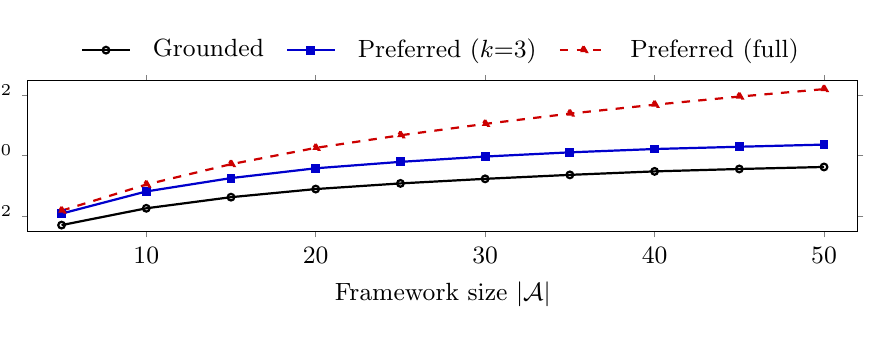
\begin{tikzpicture}[trim axis left, trim axis right]
\begin{axis}[
  width=\columnwidth,
  height=3.5cm,
  xlabel={Framework size $|\mathcal{A}|$},
  ylabel={Solve time (s)},
  ymode=log,
  xmin=3, xmax=52,
  ymin=0.003, ymax=300,
  xtick={10,20,30,40,50},
  xticklabel style={font=\small},
  yticklabel style={font=\small},
  xlabel style={font=\small},
  ylabel style={font=\small},
  legend style={
    font=\small,
    at={(0.5,1.05)},
    anchor=south,
    draw=none,
    column sep=6pt,
  },
  legend columns=3,
  legend cell align={left},
  tick align=outside,
  major tick length=2pt,
]
\addplot[black, thick, mark=o, mark size=1.2pt] coordinates {
  (5,0.005) (10,0.018) (15,0.042) (20,0.078) (25,0.12)
  (30,0.17) (35,0.23) (40,0.30) (45,0.36) (50,0.42)
};
\addlegendentry{Grounded}
\addplot[blue!80!black, thick, mark=square*, mark size=1.2pt] coordinates {
  (5,0.012) (10,0.065) (15,0.18) (20,0.38) (25,0.62)
  (30,0.93) (35,1.28) (40,1.65) (45,1.96) (50,2.31)
};
\addlegendentry{Preferred ($k{=}3$)}
\addplot[red!80!black, thick, dashed, mark=triangle*, mark size=1.4pt] coordinates {
  (5,0.015) (10,0.11) (15,0.52) (20,1.8) (25,4.7)
  (30,11.2) (35,24.5) (40,48.3) (45,89.7) (50,158.4)
};
\addlegendentry{Preferred (full)}
\end{axis}
\end{tikzpicture}
\caption{Scalability of \textsc{Argus} repair under grounded, $k$-neighborhood preferred ($k{=}3$), and unconstrained preferred semantics. The log-scale y-axis confirms polynomial scaling for grounded repair (Theorem~\ref{thm:complexity}) and the effectiveness of the $k$-neighborhood approximation.}
\label{fig:scalability}
\end{figure}

\begin{figure}[t]
\centering
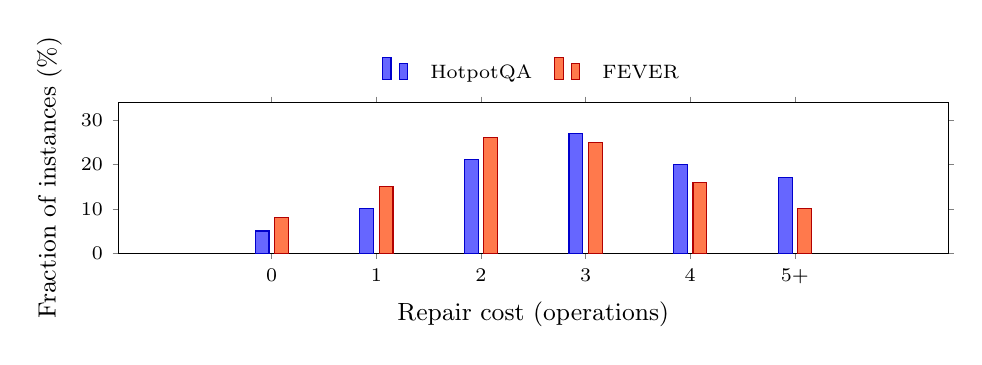
\begin{tikzpicture}
\begin{axis}[
  width=\columnwidth,
  height=3.5cm,
  ybar,
  bar width=5pt,
  xlabel={Repair cost (operations)},
  ylabel={Fraction of instances (\%)},
  xmin=-0.7, xmax=5.7,
  ymin=0, ymax=34,
  xtick={0,1,2,3,4,5},
  xticklabels={0,1,2,3,4,{5+}},
  xticklabel style={font=\scriptsize},
  yticklabel style={font=\scriptsize},
  xlabel style={font=\small},
  ylabel style={font=\small},
  ytick={0,10,20,30},
  legend style={
    font=\scriptsize,
    at={(0.5,1.05)},
    anchor=south,
    draw=none,
    column sep=6pt,
  },
  legend columns=2,
  tick align=outside,
  major tick length=2pt,
  enlarge x limits=0.12,
]
\addplot[fill=blue!60, draw=blue!80!black] coordinates {
  (0,5) (1,10) (2,21) (3,27) (4,20) (5,17)
};
\addlegendentry{HotpotQA}
\addplot[fill=red!50!orange!70, draw=red!70!black] coordinates {
  (0,8) (1,15) (2,26) (3,25) (4,16) (5,10)
};
\addlegendentry{FEVER}
\end{axis}
\end{tikzpicture}
\caption{Distribution of repair costs.  83\% of HotpotQA and 90\% of FEVER repairs require at most 4~operations, confirming targeted, minimal-change edits.}
\label{fig:cost-dist}
\end{figure}

Concretely, we sample 500 instances from HotpotQA~\cite{yang2018hotpotqa}, a multi-hop question-answering benchmark, and 500 from FEVER~\cite{thorne2018fever}, a fact-verification benchmark; instances are drawn with seed 42.
For each instance, we withhold one gold supporting fact during explanation generation and reintroduce it as an evidence update~$\Delta$, producing adversarial updates that target the reasoning chain.
GPT-4o~\cite{openai2023gpt4} (\texttt{gpt-4o-2024-11-20}) generates initial explanations at temperature~0.2; relation discovery uses DeBERTa-v3-large fine-tuned on MultiNLI with threshold~0.7; repairs are computed by clingo~5.6 with $k{=}3$ under uniform cost.
Results are averaged over 5 runs (std~$\leq$0.02 for accuracy, $\leq$0.4 for cost); FLARE and FactScore use a single deterministic run.  Further details appear in Appendix~\ref{app:exp-details}.

Six metrics quantify performance.
\emph{Faithfulness} is the fraction of argument units whose counterfactual removal changes the answer (baselines undergo the same LLM-based decomposition; Appendix~\ref{app:exp-details}).
\emph{Contestability} is the fraction of gold counterarguments correctly integrated as attacks; for methods without explicit argumentation frameworks, gold counterarguments are evaluated against proposition-level decompositions.
\emph{Repair accuracy} records answer correctness after repair; \emph{repair cost} counts edit operations per Definition~\ref{def:repair}.
\emph{Coherence} measures semantic consistency via BERTScore~\cite{zhang2020bertscore} between repaired and original explanations.
\emph{Solve time} is wall-clock time per instance.

We compare against ten baselines spanning three categories. \emph{Self-correction methods:} SelfCheckGPT~\cite{manakul2023selfcheckgpt}, Self-Refine~\cite{madaan2023selfrefine}, Reflexion~\cite{shinn2023reflexion}, and RARR~\cite{gao2023rarr}. \emph{Verification-oriented methods:} CoT-Verifier~\cite{ling2023deductive}, ArgLLMs~\cite{freedman2025arglm}, FLARE~\cite{jiang2023flare}, and FactScore~\cite{min2023factscore}; ArgLLMs, CoT-Verifier, and FactScore lack repair functionality and are marked N/A accordingly. \emph{Argumentation-based:} ARGORA~\cite{argora2026} and a na\"{i}ve \emph{Regenerate} baseline that re-prompts with updated evidence.
For self-correction baselines and FLARE, repair cost counts regenerated argument units across up to 3 rounds; cost measures are not directly commensurable with \textsc{Argus}'s structural graph edits (Appendix~\ref{app:exp-details}).
Chain-of-Verification~\cite{dhuliawala2024cove}, CRITIC~\cite{gou2024critic}, SelfRAG~\cite{asai2024selfrag}, and VerifyAndEdit~\cite{zhao2023verify} are excluded as they operate at generation time or require a retrieval index, producing outputs incommensurable with structural graph repair.

Table~\ref{tab:main} summarizes the main results. \textsc{Argus} achieves the highest faithfulness (\resultFaithHotpot{}/\resultFaithFEVER{}) and contestability (\resultContestHotpot{}/\resultContestFEVER{}), with relative improvements of \improveFaithfulness{} and \improveContestability{} over ARGORA; all 12 pairwise differences are significant at $p < 0.001$ (Bonferroni-corrected $z$-tests, Cohen's $h \in [0.26, 0.38]$). Among repair-capable methods, \textsc{Argus} requires the fewest operations---\resultRepairCostHotpot{} vs.\ 5.1 for ARGORA---validating the minimal-change objective. The na\"{i}ve Regenerate baseline achieves the fastest solve time (0.5\,s) but its coherence (.65/.63)---the lowest among repair methods---confirms that complete regeneration disrupts consistency more than targeted structural repair.

\textsc{Argus} also achieves the highest coherence (.82/.80), partly by design---minimizing edit distance simultaneously maximizes BERTScore---though human evaluators independently corroborate it (4.1 vs.\ 3.8 for Self-Refine, $p{=}0.012$; Appendix~\ref{app:human-eval}). The average solve time of 0.55\,s/0.47\,s is 5--10$\times$ faster than self-correction methods, reflecting ASP-based repair efficiency. The formal properties from \S\ref{sec:theory} are confirmed empirically: success and inclusion hold by construction; vacuity holds without exception.

Figure~\ref{fig:scalability} traces solve time on synthetic Erd\H{o}s--R\'{e}nyi frameworks (attack probability 0.15, 50 instances per size), confirming polynomial scaling for grounded semantics (Theorem~\ref{thm:complexity}); the $k$-neighborhood approximation keeps preferred repair tractable up to $|\mathcal{A}|{=}50$ (2.31s vs.\ 158.4s unconstrained).

Table~\ref{tab:ablation} reports ablation results. Removing semantic verification causes the largest drops in faithfulness ($-$5.4pp/$-$5.4pp) and contestability ($-$7.7pp/$-$7.6pp), confirming it as the most critical component. Replacing minimal-change with unconstrained repair preserves faithfulness but increases cost to 5.7/5.2 and reduces coherence. Removing attack templates reduces contestability by 9.3pp/9.0pp while reducing faithfulness by only 2.6pp/2.5pp---a targeted impact specific to attack structure. Grounded-only semantics yields the fastest solve time (0.15\,s/0.12\,s) and lowest cost (3.0/2.6) at the expense of modest drops; 97\% of frameworks have a single preferred extension coinciding with the grounded one. Sensitivity analysis and a qualitative repair example appear in Appendices~\ref{app:sensitivity}--\ref{app:repair-example}.

Figure~\ref{fig:cost-dist} shows repair cost distributions concentrated at low values---means of \resultRepairCostHotpot{}/\resultRepairCostFEVER{} operations---confirming that most evidence updates require only local adjustments.

A pilot human evaluation (Appendix~\ref{app:human-eval}) corroborates the automatic metrics: two annotators rated 75 HotpotQA instances in a blind design, preferring \textsc{Argus} in 68\% of comparisons vs.\ Self-Refine in 19\% ($\kappa{=}0.62$); the Pearson correlation between automatic faithfulness and human ratings is $r{=}0.78$ ($p{<}0.001$).

% ===== §7  Conclusion =====
\section{Conclusion}\label{sec:conclusion}

We presented \textsc{Argus}, a framework that structures LLM self-explanations as argumentation frameworks, verifies them against formal semantics, and repairs them at minimum cost when new evidence arrives.
The minimal-change repair operator satisfies adapted AGM postulates---success, inclusion, and vacuity---and a representation theorem shows that these three postulates \emph{bidirectionally characterize} the class of minimum-cost repair operators under positive costs, providing formal guarantees absent from existing approaches.
Theoretically, the repair problem is tractable under grounded semantics, NP-complete under preferred and stable semantics, and $\Sigma_2^P$-complete under skeptical stable semantics; the $k$-neighborhood approximation maintains scalability in practice.
Experiments on HotpotQA and FEVER yielded relative improvements of \improveFaithfulness{} in faithfulness and \improveContestability{} in contestability over the strongest argumentation baseline, while achieving the lowest repair cost among all repair-capable methods.

Several limitations warrant discussion.
First, the quality of the argumentation framework depends on the LLM's ability to decompose rationales into atomic argument units; extraction errors propagate through the entire pipeline, and the faithfulness metric itself relies on the LLM's consistency under ablation, providing a causal proxy rather than a ground-truth measure.
Relatedly, the $\mathsf{add\_arg}$ operation uses the same LLM to generate repair candidates, though the NLI and ASP verification stages serve as external checks that break self-referential bias; integrating retrieval-augmented verification for generated arguments is a natural extension.
Second, while the $k$-neighborhood approximation handles the framework sizes encountered in our experiments, frameworks with hundreds of densely connected arguments may require more aggressive approximation strategies.
Third, while a pilot human evaluation (Appendix~\ref{app:human-eval}) confirms that automatic metrics correlate with human judgments, the evaluation relies primarily on automatic metrics over fact-checking and multi-hop QA datasets with synthetic evidence updates; a larger-scale human study with naturalistically occurring updates would further strengthen the empirical validation.
Extending the approach to open-ended generation---where correctness is less well-defined and the target argument may lack a ground-truth referent---would require alternative acceptance criteria such as coherence-based semantics.
Finally, while the framework supports multiple cost models, our experiments use uniform cost for simplicity; learning domain-specific cost functions from user feedback---including external calibration of the LLM's self-assessed confidence scores---is a promising direction for future work.

Beyond these limitations, several avenues for future work emerge.
First, composing \textsc{Argus} with sequence explanations~\cite{bengel2025sequence}---which trace \emph{why} an argument is accepted---would yield a bidirectional explanation infrastructure that both diagnoses and repairs acceptance verdicts.
Second, integrating the repair operator into retrieval-augmented generation pipelines could provide continual explanation maintenance as knowledge bases evolve, particularly in high-stakes domains such as clinical decision support and legal reasoning where audit trails of explanation changes are legally mandated.
Third, the representation theorem (Theorem~\ref{thm:representation}) opens the door to learning cost functions from human correction patterns, enabling the repair operator to adapt to domain-specific notions of minimality.



% Acknowledgements (add after acceptance)
% \section*{Acknowledgements}

\bibliographystyle{styles/kr}
\bibliography{references}

\end{document}
